\part{Previous Systems}

The previous year's avionics systems are used to guide this years designs. This section will briefly cover the flaws
oflast year's systems to provide background on the decisions made this year.

\section{Flight Computer \& Transmitter}

The flight computer unit designed in the 2023-2024 academic year was endearingly referred to as the "QNX Stack" due to
its on-board \gls{mcu} running the \gls{qnx} \gls{rtos}. The assembled version of the unit which was flown at \gls{sac}
is pictured in Figure \ref{fig:preflight-stack}.

\subsection{Hardware Design}

The most glaring issue with the hardware design from last year was the selection of the Raspberry Pi 4B as the primary
computer for the system. The two largest issues with the Raspberry Pi were it's high power consumption and large
mechanical size. It was not an \gls{mcu}, but a full processor system with four cores and many unnecessary peripherals
like Ethernet ports, USB ports, an audio jack and HDMI ports.

The high power consumption resulted in the system only having around 8 hours of battery life, even with
\qty{4000}{\milli\ampere\hour}. Although this number is already well below the idea battery life it could have been even
lower depending on the task being performed. This is because the power consumption of a Raspberry Pi (like most
processor systems) is highly dependent on the task being performed. Were the Pi performing more demanding tasks the
battery life could have gotten as low as 2 hours or less. This became a major problem when the system would routinely
be powered on the launch pad for at least two hours before the rocket could be launched.

The large mechanical size of the Raspberry Pi was also a major issue. The Raspberry Pi is a relatively large single
board computer with many unused ports and connectors. Most of the features on this board were not used nor beneficial
for the telemetry system and unnecessarily increased the size of the system to a point where it was extremely difficult
to fit in the nosecone of the rocket.

\subsection{Enclosure Design}

The avionics enclosure was designed as a stack-up of \gls{srad} \glspl{pcb}. It was made out of aluminum to be
lightweight, with 3D printed rails and battery compartment made out of ABS filament. The enclosure sat within the
rocket's fibreglass nosecone (for radio transparency), mounted to an aluminum bulkhead. The \glspl{pcb} themselves were
held in place using a threaded rod. Screw switches to arm both the \gls{srad} system and \gls{cots} Featherweight GPS
were mounted to the side of the enclosure with 3D printed shelves.

\subsubsection{Radio Signal Integrity}

The placement of the antennas on the \gls{qnx} stack was not optimal. As can be seen in Figure
\ref{fig:preflight-stack}, the signal radiation from the longer transmitter antenna is partially blocked by the metal
enclosure, which affected transmission distance (discovered in later testing). The enclosure's reflective aluminum
material also increased signal interference, affecting the radiated signal that was not blocked but radiated forwards.
The \gls{gps} antenna (bright orange) also experienced blockage by the enclosure, resulting in a longer time to achieve
a fix.

Such a design impeded the ability of the system to transmit telemetry data and receive satellite \gls{gps} positioning
data. In particular, this would drastically reduce the signal quality received by the downlink ground station during
180 degrees of the rocket's roll, since the unobstructed portion of the antenna's radiation pattern would be facing
away from the receiver during that time.

\begin{figure}[H]
    \center
    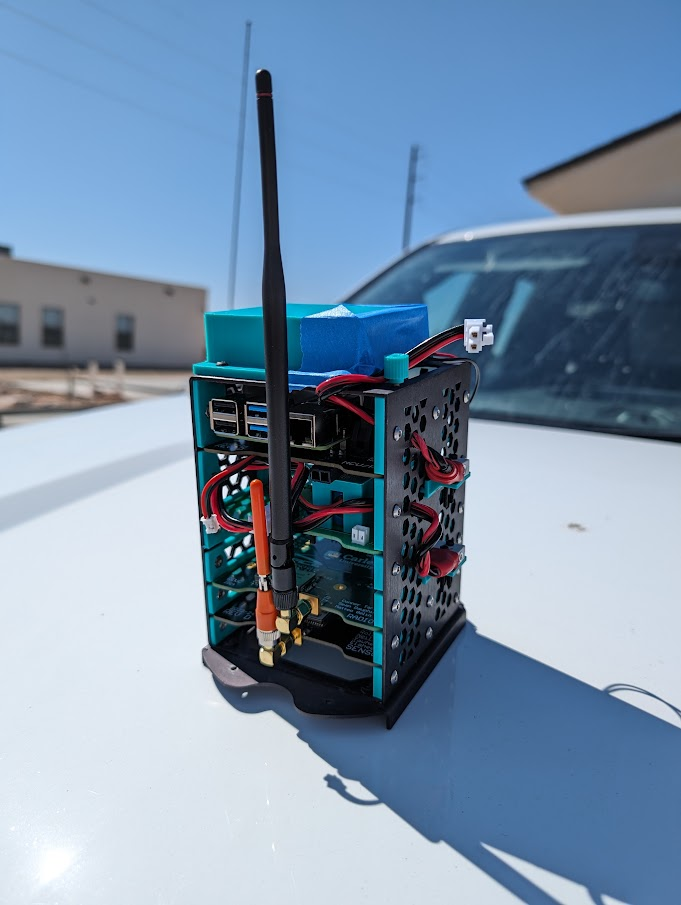
\includegraphics[width=3in]{assets/images/stack.jpg}
    \caption{The 2023-2024 avionics flight computer unit, "QNX Stack"}
    \label{fig:preflight-stack}
\end{figure}

\subsubsection{Sizing}

The QNX stack enclosure was sized in order to fit the largest member: the Raspberry Pi 4B mounted on a \gls{srad}
\gls{mcu} board. \Glspl{pcb} were sized to 90mm by 90mm, which the enclosure accommodated. This large size was
extremely tightly toleranced with the aluminum mounting bulkhead in order to fit within the rocket diameter. Figure
\ref{fig:stack-bulkhead} shows the mounting bulkhead around the enclosure.

Although initial fit-testing with \gls{cad} models was successful, the \gls{cad} model of the \gls{qnx} stack did not
include the antennas, or externally attached wiring with connectors for the electrical arming system. Figure
\ref{fig:stack-bulkhead} shows one of these connectors for supplying power to the system as it comes in contact with
the mounting bulkhead at the location where the \gls{qnx} stack was to be mounted using screws.

This connector, and the reasonably stiff wires it connects to, exceeded the clearance between the stack and bulkhead.
When the stack was inserted into the rocket nosecone, it required a series of twists and some gentle (perhaps not quite
so gentle) pressure in order to clear the bulkhead so the arming wiring connectors and antennas slid between the
threaded hole locations on the bulkhead. In fact, because this was discovered so close to the \gls{sac} flight, the
final system required the connector in Figure \ref{fig:stack-bulkhead} to be bent downward to clear the bulkhead.
Although this worked, it is not favourable to place mechanical stress on an electrical connector, much less one
responsible for arming the entire telemetry system.

\begin{figure}[H]
    \center
    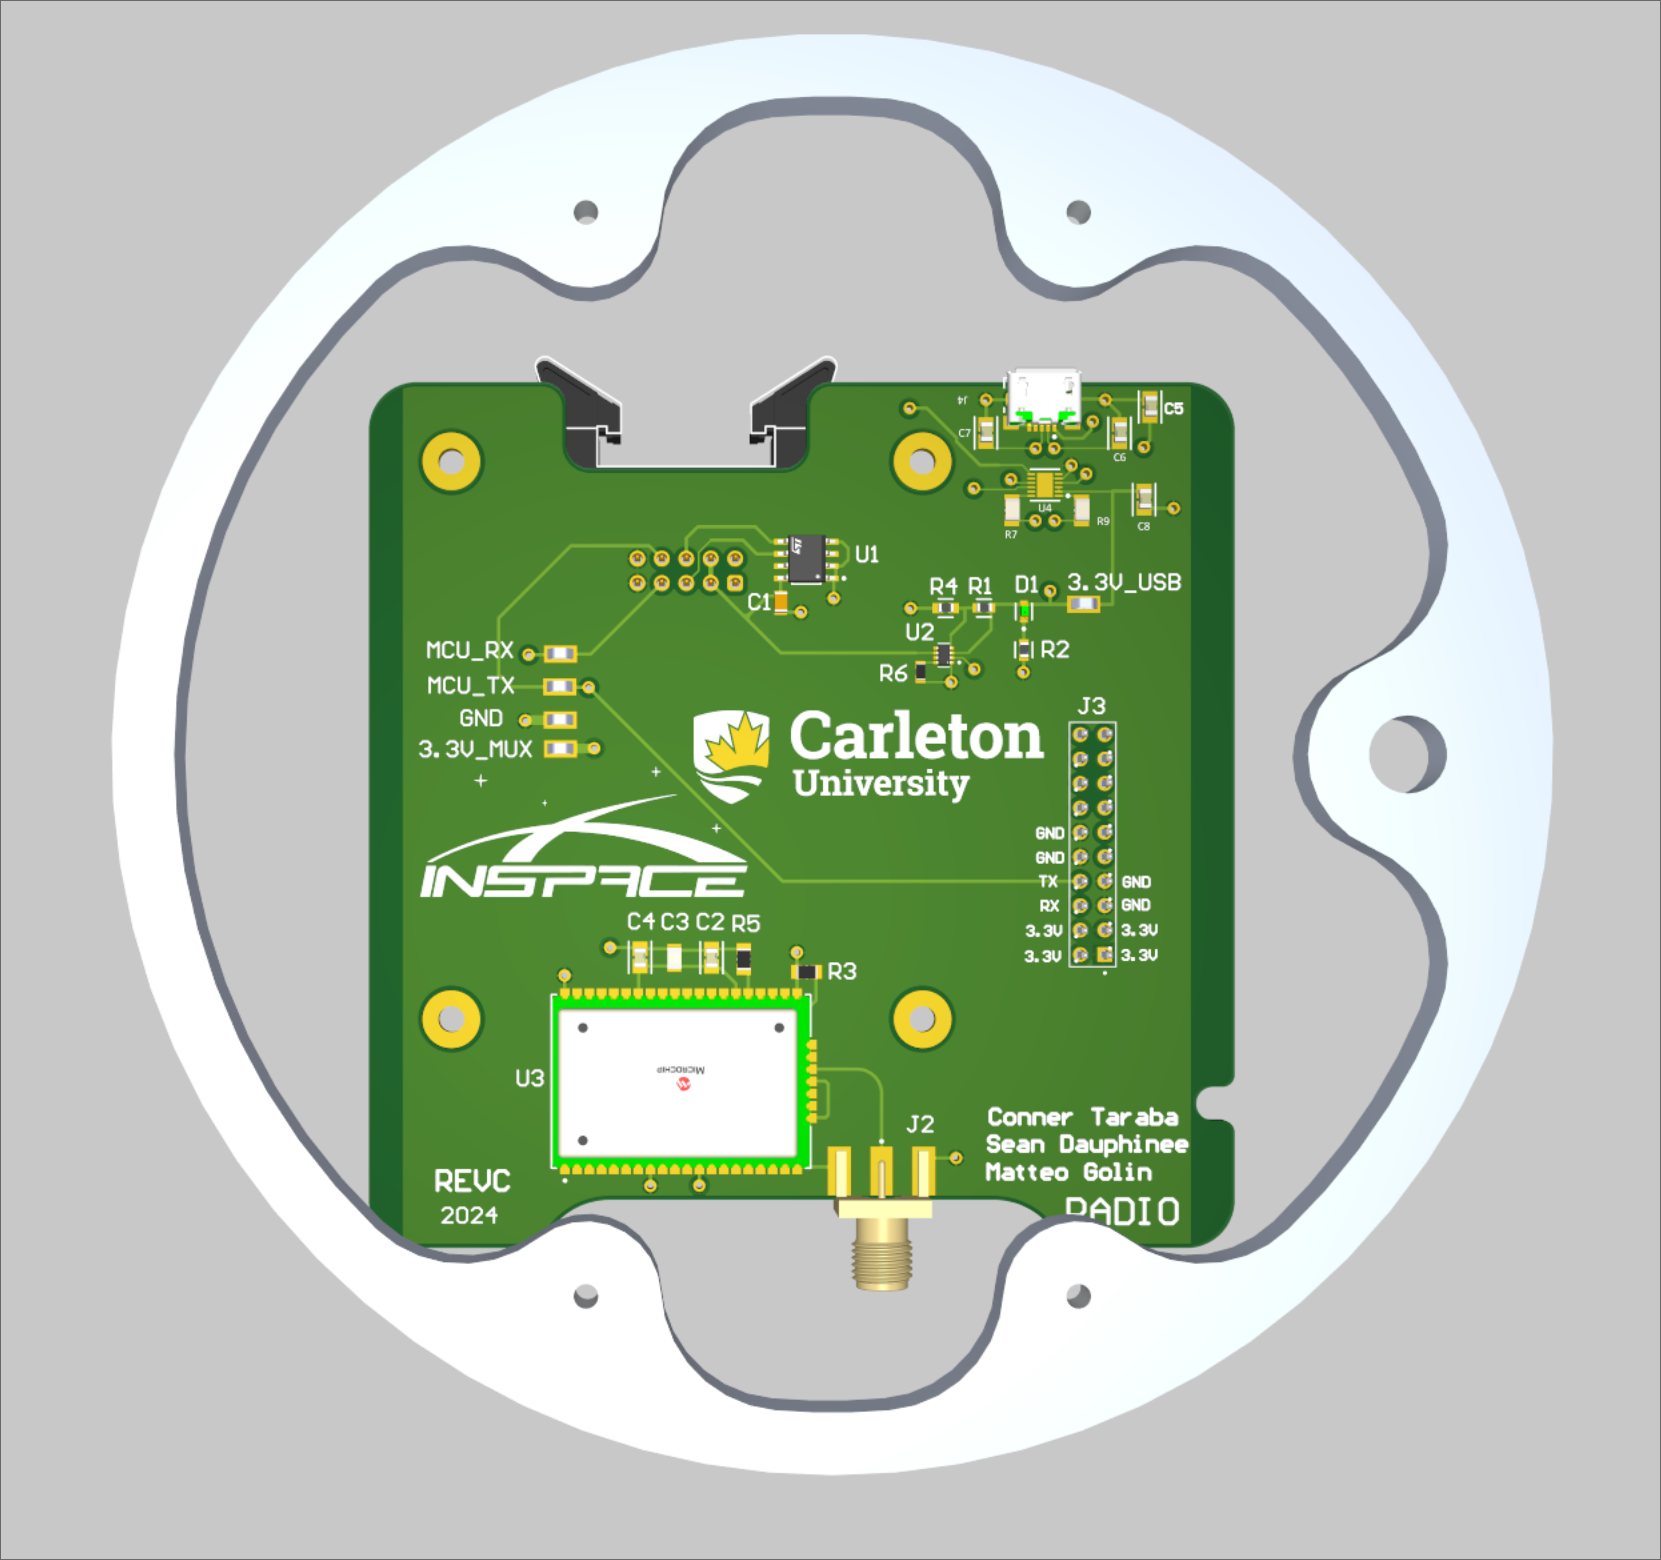
\includegraphics[width=3in]{assets/images/rad-cad.png}
    \caption{A CAD model of the radio board measured against the mounting bulkhead}
    \label{fig:rad-cad}
\end{figure}

The bulkhead clearance problem is also the reason for the close antenna placement shown in \Cref{fig:preflight-stack}.
Any further spacing between the antennas would prevent them from clearing the bulkhead due to the protruding mounting
holes on either side. A \gls{cad} visualization of this problem can be seen in \Cref{fig:rad-cad}. In fact, 90 degree
\gls{sma} connector adapters were used on the final system because the 90 degree bend on the antennas themselves
extended too far, causing them to hit the bulkhead edge when the stack was lowered into the nosecone.

\begin{figure}[H]
    \center
    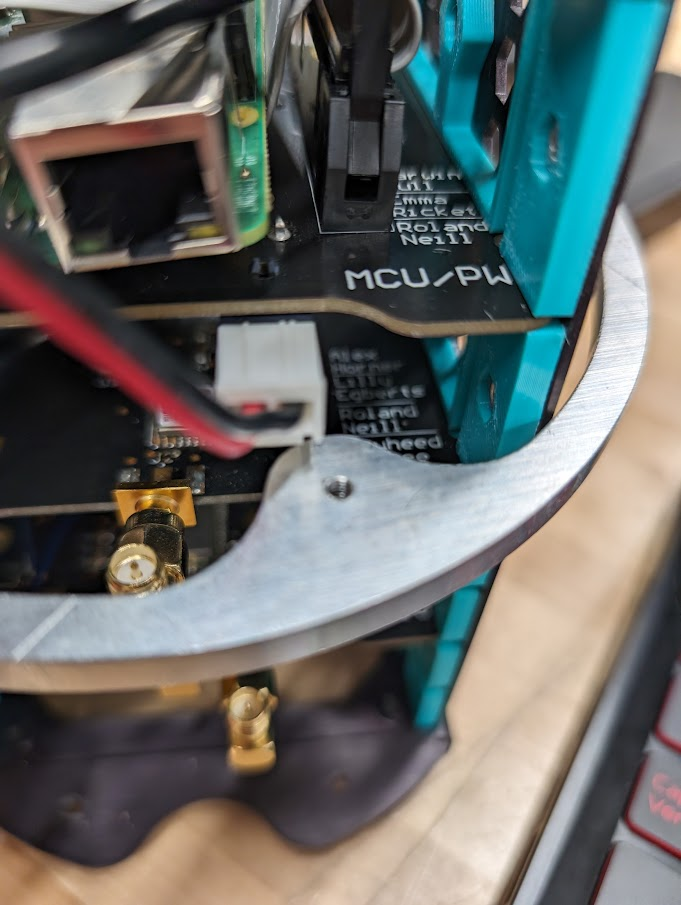
\includegraphics[width=2.5in]{assets/images/stack-bulkhead.jpg}
    \caption{The enclosure within the aluminum bulkhead ring to which it was mounted}
    \label{fig:stack-bulkhead}
\end{figure}

The enclosure of the QNX stack exhibited buckling when it was recovered post-flight. The bent shape required that the
supporting bulkhead be shaved down with a dremel tool in order to extract it. The buckling is visible
\Cref{fig:stack-bent}. All boards survived despite the buckling pushing apart the 3D-printed rails far enough for the
boards to come loose. No simulation of the enclosure was performed in advance of flight, which may have predicted these
structural problems under shock load from launch and parachute deployment.

\begin{figure}[H]
    \center
    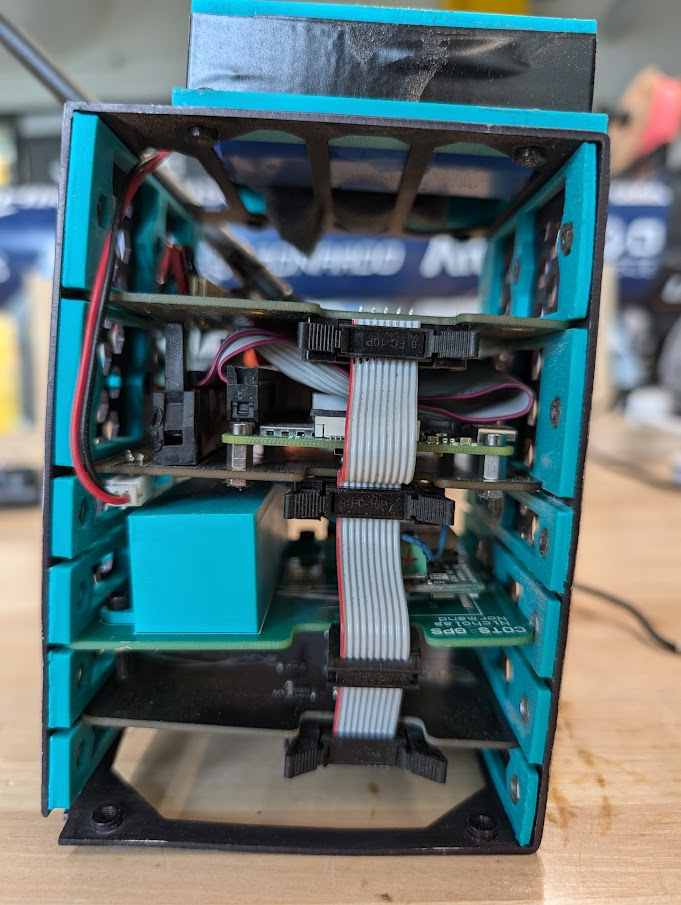
\includegraphics[width=3in]{assets/images/bent-stack.jpg}
    \caption{The recovered QNX stack post-flight, exhibiting buckling}
    \label{fig:stack-bent}
\end{figure}

\subsection{Software Design}

From a software perspective, last year's telemetry transmitter was very minimal in the quality of data that were
transmitted.

Transmitted packets contained data read directly from the onboard sensors, performing no additional sensor fusion to
measure different states of the rocket outside of using the altitude calculation suggested by the barometric pressure
sensor data sheet for combining temperature and pressure. This resulted in noisy measurements about rocket state, like
current altitude and angular velocity.

In addition, the system contained three sensors capable of measuring temperature. These sensors had a very high
measurement frequency, and were being read as fast as possible using a 1.8GHz clock speed on a Raspberry Pi 4. This
resulted in an overwhelming amount of temperature data being logged compared to other more important measurements such
as altitude, acceleration and \gls{gps} position. This also meant much of the data being transmitted over radio was
temperature data. The system design guaranteed that \gls{gps} data would always be sent when obtained because the
\gls{gps} data was measured at only 10Hz, but this guarantee was never extended to other types of data.

The system was not robust in the way it handled failures. If the system had trouble detecting the \gls{eeprom} on the
\gls{i2c} bus with startup configuration parameters, it would exit with a failure immediately instead of re-attempting
to connect or provide an external indication to the operator that something went wrong with the electrical connection
(no LED indication or buzzer, etc). This lack of robustness also applied to the radio's control process, which would
fail if it could not connect to the radio module over \gls{uart}.

The system performed logging at its maximum frequency as soon as it was armed, which caused a significant amount of
storage to be used for logging while the rocket was sitting idle on the launch pad. Although storage memory was not
scarce with last year's system (which used a 128GB SD card), it did increase power consumption during the rocket's idle
period. It is also inconvenient to sift through all the logs from the rocket's idle state in order to get the actual
flight data.

Finally, there was no indication of battery life ever implemented on this system. The driver for the current/voltage
sensor on-board was not completed in time for launch, so it was not possible to receive battery life warnings over
telemetry or through a visual indicator in the final system.
